\subsection{Electrostatic Shields: Enhancing Antenna Performance!}

\begin{tcolorbox}[colback=gray!10, colframe=black, title=E9H04] 
What is the purpose of placing an electrostatic shield around a small-loop direction-finding antenna? \\

\begin{enumerate}[label=\Alph*.]
    \item It adds capacitive loading, increasing the bandwidth of the antenna.
    \item \textbf{It eliminates unbalanced capacitive coupling to the antenna’s surroundings, improving the depth of its nulls.}
    \item It eliminates tracking errors caused by strong out-of-band signals.
    \item It increases signal strength by providing a better match to the feed line.
\end{enumerate} \end{tcolorbox}

\subsubsection{Related Concepts}

The purpose of placing an electrostatic shield around a small-loop direction-finding antenna primarily relates to electromagnetic theory and the effects of capacitive coupling. In radio communication and antenna design, the performance of antennas can be significantly affected by their environment. For small-loop antennas, unbalanced capacitive coupling can lead to inaccuracies in direction-finding and can distort the received signal.

The electrostatic shield serves as a barrier that prevents external electromagnetic fields from influencing the performance of the antenna. By having a shield, the capacitive coupling that might arise from nearby objects or other electronic devices is minimized. This greatly improves the depth of nulls in the antenna's pattern, making it more precise in determining the direction of signals.

\subsubsection{Calculation and Diagrams}

In this context, although no numerical calculations are strictly necessary, one can illustrate the concept with a simple diagram showing an antenna with and without an electrostatic shield.

\begin{center}
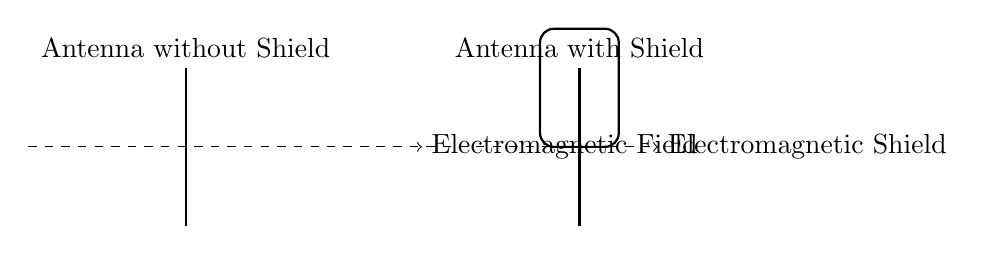
\begin{tikzpicture}
    % Draw the antenna without a shield
    \draw[thick] (0,0) -- (0,2) node[above] {Antenna without Shield};
    \draw[->, dashed] (-2,1) -- (3,1) node[right] {Electromagnetic Field};

    % Draw the antenna with a shield
    \draw[thick] (5,0) -- (5,2) node[above] {Antenna with Shield};
    \draw[thick,rounded corners=5pt] (4.5, 1) rectangle (5.5, 2.5);
    \draw[->, dashed] (2,1) -- (6,1) node[right] {Electromagnetic Shield};
\end{tikzpicture}
\end{center}

In summary, understanding the role of electrostatic shields in antenna performance is crucial for improving direction-finding accuracy and ensuring that antennas operate effectively in diverse electromagnetic environments.
